\chapter{Heavily censored lifetime data}\label{chap:chapter2}

Computerised maintenance management systems (CMMS) such as SAP \citep{sap} are now embedded in companies maintenance procedures, meaning that these companies now posses large scale datasets of component installation and replacement times. A natural use of these personalised failure time data sets is for tailoring replacement strategies for the companies specific operating environments \citep[p. 13]{Meeker2022}, rather than solely relying on the manufacturers recommendations. One problem however, is that these large observational datasets collected through CMMS are much messier that the experimental ones used by manufacturers in traditional reliability/warranty analysis. This messiness comes about because of reporting issues, incomplete historic records, and the fact that most components are pre-emptively replaced before they fail because of the risk to production and employee safety. The result is that many of the valuable data sets stored in CMMS systems are incomplete in the form of censoring and left-truncation. Censoring is when the true lifetime of a failed component is not know but either an upper bound, lower bound, or both are known. Whereas left-truncation arises when only units that have lasted more than some truncation time are observed.

The censored and left-truncated nature of such data make what would otherwise be a very strait forward analysis far more complicated. Worse yet, the incompleteness of the data is not always obvious and mistreatment during analysis can lead to biased or miss informed results. In this part of the thesis I focus on the lifetime analysis of the idler-frame dataset shown in \ref{sec:industry-data}. In this case, right censoring arises due to the set of idlers in a frame either being preventatively replace or still being in operation when the data were analysed. A portion of the lifetimes are also left-truncated, since any idlers that were installed and failed before $t_\text{start}$, when failures started being recorded in the CMMS, are not captured in the dataset. Treatment of right censored and left-truncated data was addressed by \citet{hong2009}. A further complicating factor of the idler frame dataset is that the installation time of idler-frames that were already in operation when data started being captured in the CMMS are unknown, meaning that the left-truncated lifetimes are also censored and have unknown truncation times. This issue is sometime referred to as unknown initial conditions \citep{} or unknown exposure history \citep{}. In this chapter, I propose a method for handling such cases in a Bayesian framework by imputing censored lifetimes and along with them, the truncation times.

Incompleteness of a dataset due to censoring and truncation increase uncertainty in lifetime analysis, particularly with respect to the upper tail of the lifetime distribution, since the data only contains partial information about the longer lifetimes. To improve analysis, domain knowledge can be used to fill the gap left by censoring, however only if the prior is constructed properly to do so. \citet{kaminskiy2005} propose a method for constructing a joint prior for the two parameters of the Weibull distribution by eliciting domain expert knowledge on the CDF\ldots

In this chapter of the thesis, I show how right censored and left-truncated lifetimes with unknown exposure history can be handled using fully a Bayesian treatment, and how the methods of \citet{kaminskiy2005} for developing a joint prior for the two parameters of the Weibull distribution can be incorporated into the model to supplement the analysis with additional sources of information and hence `fill in the gaps' left by the incomplete lifetime data. In this chapter I demonstrate the proposed methods using fictitious lifetime data simulated from known parameter values in a way that emulates the idler frame lifetime data to show that the method is capable of reclaiming the true parameter values. In the next chapter, I apply the method to the real idler frame dataset, and show how the fully Bayesian treatment has advantages for... (Follow Meekers paper on the transformers.)

In the remainder of this chapter is structured\ldots
\begin{itemize}
    \item Background on Weibull lifetime, censoring, left-truncation, left-truncation with unknown exposure history, constructing a joint prior.
    \item Demonstrate through simulation that the method accounts for the incompleteness of the data without introducing much bias.
    \item Extend the prior proposed in \citet{kaminskiy2005} and demonstrate it's usefulness in this context.
\end{itemize}


\section{Background}

Lifetime analysis, also called survival analysis, is the analysis of failure time data from a population of particular components/assets to derive the risk of failure of a component dependent on it's level of exposure (usually some form of time) and sometimes other covariates \citep{moore2016}. From here on I will use the general term unit/s to refer to individual/groups of the same asset or component. Lifetime analysis of a population of units typically takes place by first specifying a sampling distribution for the lifetimes by choosing some parametric lifetime distribution for the units and incorporating any observational characteristics of the data--for example censoring--then, estimating the parters of the distribution from failure time data using an appropriate inferential mechanism, and finally using the fitted model to derive useful reliability measures about the population which can be used to inform asset management plans. When done in a Bayesian context, the first step of this process also includes specifying a prior distribution. From the resulting inference, we can devise optimal replacement strategies that minimise the risk of unplanned failures, and hence the risk of lost production, and also the cost of the maintenance strategy.

\subsection{Lifetime distribution}

The lifetimes of the units are modelled as a random variable defined in terms of $t$, the exposure time, on $[0, \infty)$. $t$ is some continuous or discrete exposure time from a clearly defined origin, the installation of the component, to a well defined event, the failure of the component. In reliability analysis, the exposure is typically absolute time, the operating time of the unit, or cycles of operation. In this analysis I use absolute time since operating time was not available. Next, a specific parametric lifetime distribution is chosen for the random variable $t$, $p(t|\theta)$, expressed as the probability density function (PDF) and the parameters of the lifetime distribution are estimated from the data. Once the estimates are obtained, different specifications of the lifetime distribution can be used to draw useful insights in order to inform decisions:
\begin{itemize}
    \item \textbf{Cumulative distribution function} (CDF), $F(t)$, it the probability that a unit will have failed by time $T$, i.e. $P(t <= T)$. It is also sometimes called the cumulative risk function.
    \item \textbf{Survival function}, $S(t)$, is the complement of the CDF and defines the probability of a unit surviving up to an exposure time $t$.
    \item \textbf{Hazard function}, $h(t)$, which is the instantaneous failure rate, i.e. the probability that given a unit has survived up to time $T$ it will fail in the next small interval.
\end{itemize}
For example, the CDF quantifies the risk of unplanned failures given a chosen preventative maintenance interval, and the Hazard function identifies if a units risk of failure increases as it ages and therefore if a preventative maintenance strategy is even suitable at all.

\subsection{The Weibull distribution}

In the analysis that follows, I use the Weibull distribution to model the idler frame lifetimes, that is
\begin{equation}
    y|\beta, \eta \sim \hbox{Weibull}(\beta, \eta),
\end{equation}
where $\beta$ is the shape parameter and $\eta$ is the scale. The Weibull distribution is a commonly used lifetime distribution because of its ability to capture an increasing, constant, or decreasing risk of failure. In addition, the weibull distribution is the limiting distribution for the minimum value in a sample when the sample space is lower bounded; such as lifetimes, which must be greater than zero. This characteristic of the weibull distribution gives it a convenient interpretation in component reliability; the lifetime of a unit is the time of the first occurring catastrophic failure mode of the unit. In my analysis that follows, I use the coupled parameterization of the two-parameter Weibull distribution, which has PDF
\begin{equation}
    f(t) = \frac{\beta}{\eta}\left(\frac{t}{\eta}\right)^{\beta - 1} \exp^{-\left(\frac{t}{\eta}\right)^{\beta}},
\end{equation}
CDF
\begin{equation}
    F(t) = 1 - \exp^{-\left(\frac{t}{\eta}\right)^{\beta}},
\end{equation}
and hazard function
\begin{equation}
    h(t) = \frac{\beta}{\eta}\left(\frac{t}{\eta}\right)^{\beta - 1}.
\end{equation}
The shape parameter $\beta$ dictates whether the hazard increases, $\beta > 1$, decreases, $\beta < 1$, or stays constant, $\beta = 1$. The effect of the shape parameter on the hazard function is demonstrated in \textit{Figure}~\ref{fig:hazard_function_demo}. Practically speaking, if the hazard function increases with exposure, then this corresponds to a wear out failure mechanism, where as if it decreases then this corresponds to infant mortality. This is important from a maintenance perspective because if the component does not wear out, then preventative replacement policy is not suitable \citep{jardine2013}. In other words, we want to be sure that $\beta > 1$ before implementing a preventative policy.

\begin{figure}[h]
    \centering
    \includegraphics[width=1\textwidth]{./figures/hazard_func_demo.pdf}
    \caption{Hazard function for $\beta = 0.9$, $\beta = 1$, and $\beta = 1.1$.}
    \label{fig:hazard_function_demo}
\end{figure}

\subsection{Censoring}

It is very common for lifetime data to be censored. Censoring occurs when we only partly observe the lifetime of a unit, or in other words we only observe upper and lower bounds for the lifetime. There are three types of censoring: left, interval, and right censoring, but all are treated in much the same why. \textit{Figure}~\ref{fig:cense_examp} demonstrates these three types of censoring. In the figure, three units are installed at time $t_0$ and then two follow up inspections are performed at times $t_1$ and $t_2$. The true, partially observed, failure times of each unit are shown as crosses in the figure. Left censoring occurs when we only observe an upper bound of the lifetime, an example is if we know the install time of a unit and observe it as failed at $t_1$ and so we only know that the true value of the lifetime must be less than $t_1$. Interval censoring occurs if we only know an upper and lower bound for the lifetime, i.e. if a unit fails between inspection times then we know that the lifetime must be greater than $t_1$ but less than $t_2$. Right censoring occurs when we only know a lower bound for the lifetime. For example, if a unit is still in operation when we perform our analysis, e.g. it has lasted longer than $t_2$, then we only know that the true value of the lifetime must be greater than $t_2$. Right and left censoring are special cases of interval censoring where the upper or lower bound of the lifetime are infinity or zero respectively. Left censoring is fairly uncommon and so In the discussions that follow, I focus on right and interval censoring but all of the methods can be easily extended to accommodate left censored data as well.

\begin{figure}[h]
    \centering
    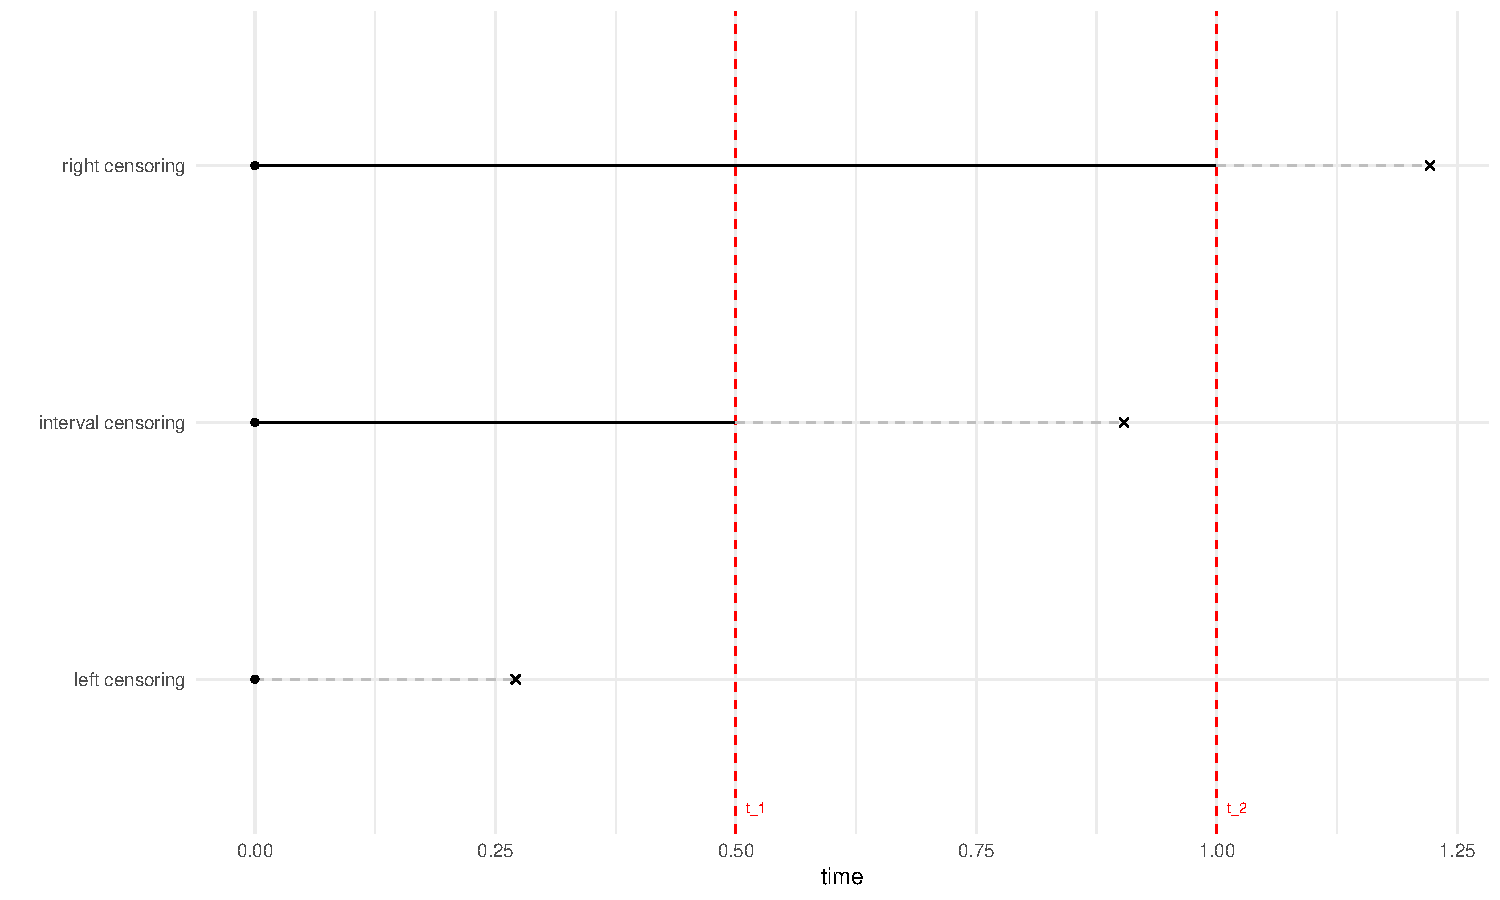
\includegraphics[width=1\textwidth]{./figures/censoring_example.pdf}
    \caption{}
    \label{fig:cense_examp}
\end{figure}

One way of handling censored data is to treat the censored lifetimes as missing data, which in a Bayesian framework is to treat them as a random variable in the model \citep[p.211]{reich2019}, and constrain their values to fall within the upper and lower censoring bounds \citep{stan_user_guide2024}. This is easily done in probabilistic programming languages like Stan. Treating the missing data as random variables in the model requires us to specify a distribution for the censored lifetimes, which we assume is the same distribution as the rest of the population,
\begin{equation}
    \label{eq:impute-cens}
    y^C_i|\beta, \eta \sim \hbox{Weibull}^{t^{\hbox{\tiny{Upper}}}_i}_{t^{\hbox{\tiny{Lower}}}_i}(\beta, \eta).
\end{equation}
Here $y^C_i$ is an unobserved censored lifetimes, and the superscript $t^{\hbox{\tiny{Upper}}}$ and subscript $t^{\hbox{\tiny{Lower}}}$ indicate that the distribution is constrained by the upper and lower censoring times. Once the missing lifetimes have been imputed, the likelihood of the observed and imputed lifetimes can be calculated in the same way as a typical lifetime dataset with no censoring. This approach of imputing the censored lifetimes is not unique to Bayesian methods. The same can be done using an Expectation Maximisation algorithm and maximum likelihood \citep{mitra2013}. However, using the Bayesian approach, along with MCMC methods, it is very simple to derive uncertainty intervals for the parameters, imputed values, and useful quantities.

An alternative approach is to simply integrate out the censored observations. The probability that a censored observation falls between the upper and lower censoring times is
\begin{equation}
    \label{eq:integrate-out-cens}
    Pr\left[t^{\hbox{\tiny{Lower}}} < y^C_i \leq t^{\hbox{\tiny{Upper}}}\right] = \int_{t^{\hbox{\tiny{Lower}}}}^{t^{\hbox{\tiny{Upper}}}} f\left(y^C_i\right) d y^C_i = F\left(t^{\hbox{\tiny{Upper}}}\right) - F\left(t^{\hbox{\tiny{Upper}}}\right).
\end{equation}
By integrating out the censored observations, the likelihood can be written as
\begin{equation}
    \label{eq:censored_likelihood}
    L\left(\theta|y^O, t^{\hbox{\tiny{Upper}}}, t^{\hbox{\tiny{Lower}}}\right) = \prod^{N^O}_{i = 1}f(y^O_i) \prod^{N^C}_{j = 1}\left[F(t^{\hbox{\tiny{Upper}}}_j) - F(t^{\hbox{\tiny{Lower}}}_j)\right],
\end{equation}
where $\theta$ are the parameters of the lifetime distribution, $N^O$ and $N^C$ are the number of fully observed and censored observations respectively, and $y^O_i$ are the fully observed lifetime. This second approach is much more commonly used, particularly in the reliability literature (). However, as I show later, for the particular problem when data are also left-truncated with unknown installation times, it is convenient to frame the model in the form of the first imputation approach.

\subsection{Left-truncation}

Truncation arises when a sample comes from an incomplete population, or in other words, there is some criteria that part of the population must appease in order to be observable \citep{guo1993}. Left-truncation, for example, arises when some units must survive up to a certain time in order to be included in the dataset. It is also possible for data to be right- or doubly-truncated, but left-truncation is the most common in lifetime data. The definition of left-truncation and left-censoring may seem very similar, however, they are distinctly different \citep{mitra2013}. Censoring is a characteristic of the sample, i.e. we know the number of left-censored observations but not the exact values of their lifetimes, whereas truncation is a characteristic of the population because we do not know how many units were not included in the dataset because they did not survive past the truncation time(the time from the installation of the unit to the start of observation) and hence our sample is not representative of the true population. An example of a left-truncated dataset is shown in \textit{Figure}~\ref{fig:left_trunc_example}. 

\begin{figure}[h]
    \centering
    \includegraphics[width=1\textwidth]{./figures/left_truncation_example.pdf}
    \caption{}
    \label{fig:left_trunc_example}
\end{figure}

In \textit{Figure}~\ref{fig:left_trunc_example}, units that were installed prior to $t_{\hbox{start}}$ come from a left-truncated distribution since any other unit that was installed at the same time but did not last until $t_{\hbox{start}}$ are not included in the sample. The left-truncated cases caused by the start of the observation period (units three, four, five, and seven in \textit{Figure}~\ref{fig:left_trunc_example}) tend to over-represent low-risk cases since any high risk case installed at the same time is absent from the sample \citep{guo1993}. Observations that arise from a left-truncated distribution can be included in the analysis by re-normalising their lifetime distribution by dividing by the probability of surviving past the truncation time;
\begin{equation}
    \label{eq:left_trunc}
    L\left(\theta|y^T_i\right) = \frac{f\left(y^T_i\right)}{1 - F\left(\tau^{\hbox{\tiny{Left}}}_i\right)},
\end{equation}
where $y^T_i$ is the left-truncated lifetime, and $\tau^{\hbox{\tiny{Left}}}_i$ is the truncation time.

\subsection{Left-truncation and right-censoring} 

A common scenario in reliability datasets is a combination of both left-truncation and right-censoring. This case naturally arises in historic observational datasets, such as those found in CMMS, where units are repeatedly replaced once they fail and any units that were installed and failed before the start of the observation process (which might be the data a new CMMS was adopted) are absent in the dataset. \textit{Figure}~\ref{fig:left_trunc_and_right_cens_example} shows a toy example of this case, where three units are repeatedly replaced when they fail and we start to observe their failures at $t_{\text{start}}$ and stop at $t_{\text{end}}$. Any lifetimes that fail before $t_{\text{start}}$ are unobserved and so are greyed out, resulting in the first observed lifetime of each unit being a left-truncated sample. Lifetimes that surpass $t_{\text{end}}$ are only partially observed (right censored), hence the portion of these lifetimes that sits to the right of $t_{\text{end}}$ is also greyed out. \citet{hong2009,mitra2013,kundu2016} analyse a dataset of electrical transformer failures that follows this general structure and \citet{mittman2013} looks at a similar case for computer hard drives. The idler frame failure data is also an example of this type of dataset.

\begin{figure}[h]
    \centering
    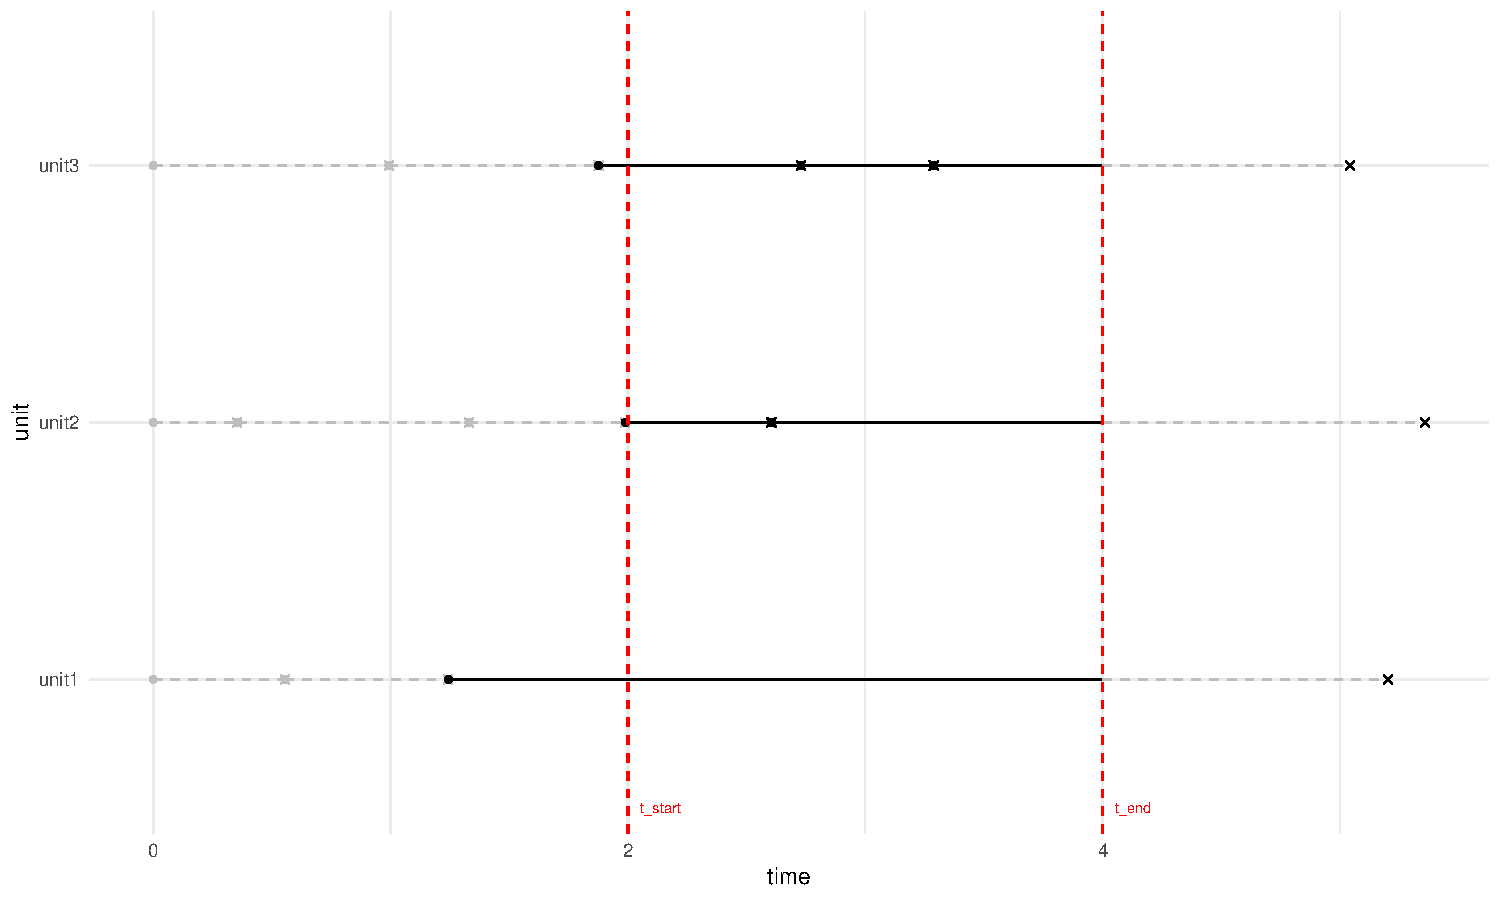
\includegraphics[width=1\textwidth]{./figures/left_truncation_w_right_censoring_example.pdf}
    \caption{}
    \label{fig:left_trunc_and_right_cens_example}
\end{figure}

\citet{hong2009} shows how a likelihood for data that is left-truncated and right-censored can be constructed using the general approach of integrating out the censored observations,
\begin{equation}
    \label{eq:left_trunc_and_right_cens_int}
    L\left(\theta|y^O, t^{\hbox{\tiny{Lower}}}, \tau^L_i\right) = \prod^{N^O}_{i = 1}\left[\frac{f(y^O_i)}{1 - F(\tau^L_i)} \right] \prod^{N^C}_{j = 1}\left[\frac{1 - F(t^{\hbox{\tiny{Lower}}}_j)}{1 - F(\tau^L_j)}\right],
\end{equation}
where $\tau^L$ are the truncation times and if the lifetime is not truncated $\tau^L = 0$. \citet{kundu2016} then implements the same approach in a Bayesian framework using a gibbs sampling algorithm to draw samples from the posterior. \citet{mitra2013} takes the alternative approach of imputing the censored lifetimes using an expectation maximisation algorithm and the complete data likelihood
\begin{equation}
    \label{eq:left_trunc_and_right_cens_imp}
    L\left(\theta|y^O, \hat{y}^C, \tau^L_i\right) = \prod^{N^O}_{i = 1}\left[\frac{f(y^O_i)}{1 - F(\tau^L_i)} \right] \prod^{N^C}_{j = 1}\left[\frac{f(\hat{y}^C_j)}{1 - F(\tau^L_j)}\right],
\end{equation}
where the $\hat{y}^C_j$ are the imputed values of the censored observations. I express the same approach as \ref{eq:left_trunc_and_right_cens_imp} in a Bayesian framework as
\begin{align*}
    y^O_i|\beta, \eta & \sim \hbox{Weibull}(\beta, \eta) \quad T[\tau^L_i, ]\\
    y^C_j|\beta, \eta & \sim \hbox{Weibull}_{t^{\hbox{\tiny{Lower}}}_j}(\beta, \eta) \quad T[\tau^L_j, ] \\
    \beta, \eta & \sim \pi(\theta_{\beta, \eta}),
\end{align*}
where $\hbox{Weibull}_{t^{\hbox{\tiny{Lower}}}_j}$ indicates that the random variable $y^C_j$ has a Weibull distribution and is constrained to be greater than the censoring time, and $T[\tau^L, ]$ indicates that the distributions are re-normalised by the probability $P(y > \tau^L)$ (Note: I stole this notation from the stan code). For the moment, I express a joint prior for the parameters in its most general form.

\paragraph{Unknown truncation time}

A problem arises when the installation time of the left-truncated lifetimes is unknown, since to normalise the truncated lifetime distribution of the left-truncated observation $\tau^{\hbox{\tiny{Left}}}$ must be known. For example, if for the dataset shown in \textit{Figure}~\ref{fig:left_trunc_and_right_cens_example} there was no information at all prior to $t_\text{start}$, then we could not use the likelihood in \ref{eq:left_trunc_and_right_cens_int} or \ref{eq:left_trunc_and_right_cens_imp}. This is the case for the idler frame data in. This problem is referred to either as unknown exposure history () or initial conditions (). In these case, there are two approaches that can be taken \citep{guo1993}. The first, discard all of the left-truncated samples \citep{}, in which case the parameter estimates are still unbiased \citep{}. However, in doing so we throw away a large amount of information. In most cases of left-truncation and right censoring, the right censoring masks any information about longer lifetimes and so the left-truncated samples are the only source of information about the upper tail of the lifetime distribution. The second approach is to assume a constant hazard, i.e. $\beta = 1$, since in this case the Weibull distribution reduces to the exponential and, no matter the age of a unit, the probability of it surviving a given period is constant (this is the memoryless trait of the exponential distribution). However, assuming a constant hazard is very restrictive and often one of the aims of performing lifetime analysis in the first place is to determine if $\beta > 1$. Furthermore, assuming an exponential distribution when the data do not have a constant hazard may lead to severe bias in the parameter estimates \citep{heckman1986}. In \textit{Section}~\ref{}
I show how treating the unknown installation times as a case of censoring and using the method of imputing the censored data, the missing truncation times can also be imputed and reasonable parameter estimates can be obtained.

%Whereas Cases of right and interval censoring are demonstrated in \textit{Figure}~\ref{fig:censoring_example}~\textit{A}. The figure shows three units observed over a period of $5000$ to $75000$ \textit{days} of operation, indicated by the red vertical lines. The installation of the units is represented by a solid dot and its failure by a cross. Any part of the lifetimes that fall outside of the period of observation are unknown and are therefore greyed out. The lifetime of unit three is a fully observed lifetime since the unit is both installed and fails within the observation period. Unit two on the other hand was installed before the period of observation and failed while we were observing it. Unit two is therefore interval censored because we know that it's installation time must be between $t = 0$ and $t = 5000$, and we can therefore deduce that the lifetime must be between $t = 2430$ and $t = 7430$. The last case, unit one, is right censored since it was installed during the observation period and had not yet failed by the time we stopped observing it. For the case of unit one, we can only deduce that the lifetime was at least as long as we observed it for. \textit{Figure}~\ref{fig:censoring_example}~\textit{B} shows how the three case in \textit{A} arise in an experiment. \textit{B} is a simplified case of the idler frame data where there are three similar components(units) on an asset that are continuously replaced when they fail and we only start to properly record the failures after $5000$ \textit{days} of operation. This could be because a twenty year old mine site only started to use electronic maintenance management software capable of capturing the information seven years ago

\section{Imputing truncation times}

Using the toy example in \textit{Figure}~\ref{fig:left_trunc_and_right_cens_example}, say we do not observe any of the installation or failure times to the left of $t_\text{start}$. In this case, we know that the first, partially, observed lifetime from each unit started some time between $t = 0$ and $t = t_\text{start}$. This is a case of interval censoring, where the lower censoring bound is the time from the beginning of observation to the failure time and the upper bound is from $t = 0$ to the failure time. If we did not know the origin time $t = 0$ with respect to $t = t_\text{start}$ then it would be a case of right censoring, but the following logic would still apply. Let $t^{\text{failure}}_{i}$ be the failure time of the $i^{th}$ observation. Treating the observations as interval censored, the left-truncated lifetime can be imputed as in \textit{Section}~\ref{} by sampling from
\begin{equation}
    \hat{y}^L_i|\beta, \eta \sim \hbox{Weibull}^{t^{\text{failure}}_{i}}_{t^{\text{failure}}_{i} - t_\text{start}}(\beta, \eta).
\end{equation}
Using the imputed values of the lifetime it is then possible to calculate the truncation time by
\begin{equation}
    \tau^L_i = \hat{y}^L_i - \left(t^{\text{failure}}_{i} - t_\text{start}\right).
\end{equation}

A complication arises when the lifetime is both interval censored by the start of the observation period and right censored by the end, such as unit one in \textit{Figure}~\ref{fig:left_trunc_and_right_cens_example}. In this case the truncation times value is unknown but is between $\tau^L = 0$ and $\tau^L = \min\left(t_\text{start}, \hat{y}^L_i - (t_\text{end} - t_\text{start})\right)$. Since we have no reason to expect that the truncation time is not uniform, we can impute the truncation time using the uniform distribution
\begin{equation}
    \tau^L_i \sim \hbox{Uniform}(0, \min\left(t_\text{start}, \hat{y}^L_i - (t_\text{end} - t_\text{start})\right)).
\end{equation}
Sampling the value of $\tau^L_i$ in this way should incorporate the extra uncertainty in our Bayesian estimates.

\section{Informative joint prior}

In cases where data only provide partial information, such as lifetime data where some lifetimes are masked by censoring, informative priors can help to `fill in the gaps' and inform areas of the model that the data cannot. For example, right censoring masks the upper tail of the lifetime distribution, and if there are no observed failures beyond some censoring time then the data do not contain any information that informs this upper tail of the lifetime. This is clear in Section~\ref{} when I fit a Weibull distribution to censored lifetimes after discarding any truncated lifetimes. An added motivation for using an informative prior in these cases is that non-informative priors can place mass in unreasonable parts of the parameter space and when combined with a week likelihood, this leads to spurious parameter estimates \citep{tian2024}.

\citet{kaminskiy2005} proposes a method for encoding an informative joint prior for the two parameters of the Weibull distribution by eliciting information about cross sections of the weibull CDF. In the proposed method, the analyst provides their expected value of the CDF at two exposure times, $t_1$ and $t_2$, and their level of uncertainty around these estimates. The pair of estimate and uncertainty level at each exposure time $(\mu_{\hat{F}_{t_i}}, \sigma_{\hat{F}_{t_i}})$ are encoded as the mean and standard deviation of a beta distribution. By then sampling realisations of the CDF at each exposure time from the two distributions, ensuring that $\hat{F}_{t_1} < \hat{F}_{t_2}$, the parameters of the Weibull CDF that passes through the two realisations can be calculated to obtain a draw from the informative joint prior. \citet{kaminskiy2005} then show how to obtain a Bayesian point estimate of the CDF at some new exposure time where binomial failure data are available by first calculating the parameters of a new beta distribution that describes the CDF at the new exposure time using the joint prior draws and then updating the parameter estimates with the data, taking advantage of the beta-binomial conjugacy.

The method that \citet{kaminskiy2005} propose to obtain joint draws from an informative prior for the two weibull parameters falls under the recommendations of \citet{gelman_workflow_2020}, who suggest to elicit information on the outcome space---which is more familiar to partitioners---and then translate this information into an informative prior also that indirectly describes how the parameters should be allowed to covary with one another. An alternative method proposed by \citep{Meeker2022} to elicit an informative prior for the Weibull parameters is to reparameterise the distribution in terms of the shape $\beta$ and some quantile, $p_r$, of the distributions and then specify independent priors for $\beta$ and $p_r$. Both methods have proven to be useful in practice and been implemented in reliability software due to their usability \citep{Krivtsov}. However, it can be difficult to elicit information about $\beta$ for practitioners not very familiar with Weibull analysis. Therefore, I use a variation of \citeauthor{kaminskiy2005}s method for obtaining draws from a joint informative prior for the Weibull parameters and build upon their method by showing\ldots
\begin{itemize}
    \item Need to discuss Krivtsov's development of \citet{kaminskiy2005} somewhere\ldots
\end{itemize}

In their proposed procedure, the prior is updated with the data using the conjugacy of the binomial likelihood and beta prior for the CDF at the new exposure time $t_3$. Doing so only provides point estimates of the updated parameter values of the beta distribution at $t_3$. To obtain corresponding values of the Weibull parameters, the analyst must once again sample paris of realisations along the CDF---now at either $t_3$ and $t_1$ or $t_3$ and $t_2$---and calculate the parameters of the Weibull CDF that passes through the two points. In doing so they `reuse' the prior distribution at either $t_1$ or $t_2$ to generate the posterior and so the `prior belief' about the CDF at which ever time is used is not really updated at all. Furthermore, the resulting joint draws will be sensitive to weather $t_1$ or $t_2$ is used to regenerate the joint distribution of the Weibull parameters. By instead implementing the method for obtaining draws from the joint prior within the HMC sampling algorithm, I show how to properly filter the prior through the likelihood to obtain the full posterior. Doing so also means that the prior can be updated with detailed lifetime data(i.e. failure times rather than binomial trial data), censoring and truncation information can be included in the likelihood, and the resulting full posterior contains proper uncertainty quantification. 

Rather than beta distributions, I use normal distribution truncated between zero and one to encode prior belief about the CDF at $t_1$ and $t_2$. This is because when specifying prior information close to the boundary, for example if our estimate of the cdf is $0.95$ or $0.05$, with reasonable uncertainty surrounding the estimate, a beta distribution places lot of mass very close to zero or one which causes numerical issues during sampling. Truncated normal distributions are much better behaved. The prior can be expressed as
\begin{align*}
    \hat{F}_{t_1} \sim & \hbox{N}^{1}_{0}(\mu_{\hat{F}_{t_1}}, \sigma_{\hat{F}_{t_1}})             \\
    \hat{F}_{t_2} \sim & \hbox{N}^{1}_{\hat{F}_{t_1}}\left(\mu_{\hat{F}_{t_1}}, \sigma_{\hat{F}_{t_1}}\right) \\
    \beta            = & \frac{g(\hat{F}_{t_2}) - g(\hat{F}_{t_1})}{\log(t_1 / t_2)}               \\
    \eta             = & \exp\left[\log(t_1) - \frac{\hat{F}_{t_1}}{\beta}\right]
\end{align*}
where $g(\hat{F}) = \log(-\log(1 - \hat{F}))$ and the superscript and subscripts on the normal distribution indicate the upper and lower constraints of the support.

Depending on the choice of $t_1$ and $t_2$ the analyst encodes different information into the joint prior, which is reflected in how the two parameters covary with one another. For demonstration, plots (a), (b), and (c) in Figure~\ref{fig:kaminskiy-join-priors} show the draws from three different joint priors constructed using this elicitation method. To construct the prior, I specify some `true' values of the parameters $(\beta = 1.1; \eta = 1)$ and then specify the priors to reflect the true value of the CDF at different quantiles $t_i = p_r$ so that all of the priors contain the `true' parameter values. (a) shows a prior where information is encoded at early exposure times ($t_1 = p_{0.05}$ and $t_2 = p_{0.20}$), (b) shows one where information is encoded at times around the median age ($t_1 = p_{0.40}$ and $t_2 = p_{0.60}$), and (c) shows one where the elicitation times are in the upper tail of the lifetime distribution($t_1 = p_{0.90}$ and $t_2 = p_{0.99}$). Plots (d), (e), and (f) in Figure~\ref{fig:kaminskiy-join-priors} show the corresponding uncertainty around the Weibull CDF that results from the different priors in (a), (b), and (c) respectively. We see that the joint prior allows us to express our prior belief in one area of the PDF while allowing the prior to be vague in others. This characteristic has useful application in the context of heavy censoring since censoring masks longer lifetimes and hence increases uncertainty in the upper tail of the distribution, but still contains useful information in the lower tail.

\begin{figure}
    \centering
    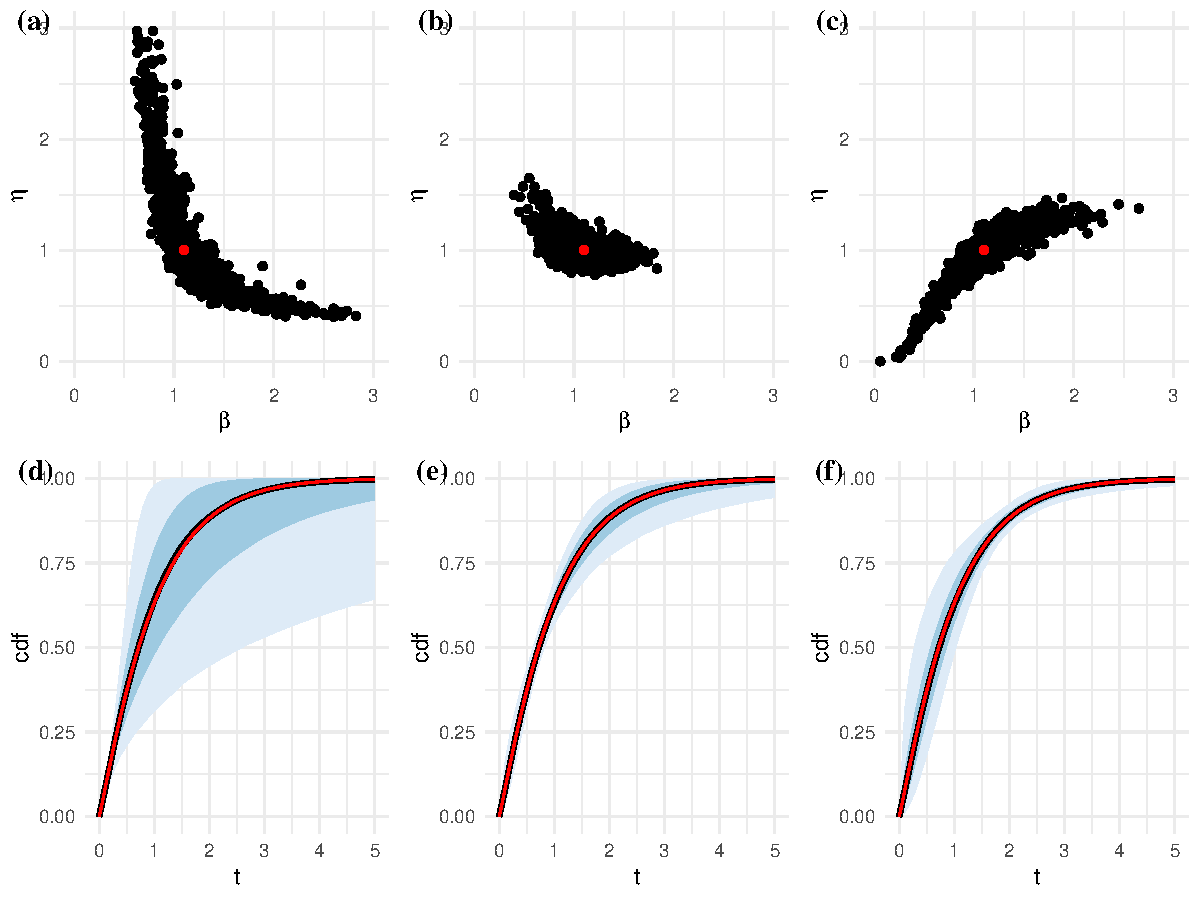
\includegraphics[width=1\textwidth]{./figures/ch-2/joint-priors.pdf}
    \caption{}
    \label{fig:kaminskiy-join-priors}
\end{figure}

In this chapter, I compare the informative joint prior shown in Figure~\ref{fig:kaminskiy-join-priors}~(c) and~(f), which encodes information in the upper tail, with the vague independent priors $\beta \sim \hbox{N}^{+}(1.1, 1)$ and $\eta \sim \hbox{N}^{+}(1, 1)$, where the superscript $(+)$ indicates that the prior is truncated to be positive. 

\section{Analysis of simulated data} \label{sec:weibull-sim-example}

\begin{itemize}
    \item Here I demonstrate the method with simulation.
    \item I simulate lifetime data in a way that emulates the observational process of the idler frame data.
    \item However, I save the installation times of observations that are left truncated by the start of the observation time.
    \item I then compare the inference of the imputation approach with the alternative where we discard all of the left censored lifetimes and also with the case where we do in fact know exposure history of the left truncated samples.
    \item For a small sample, the imputation approach gives almost the same inference as the case where we know the true installation times. When we throw out all of the left truncation times, there is a massive increase in uncertainty, particularly around the upper tail of the lifetime distribution, as shown in the posterior of the CDF.
    \item I then refit the same models to the simulated data but with an informative joint prior encoded in a away that informs the upper tail of the distribution. All of the models now give very similar results, however, the case where we discard the left truncated samples still has larger uncertainty.
\end{itemize}

%The toy example given in \textit{Figure}~\ref{fig:censoring_example}~\textit{B} is based on the Conveyor Idler Frame data introduced in \textit{Section}~\ref{sec:industry-data}. In the case of the Idler frames, the high reliability of the components when compared to length of the observation period results in heavy censoring; roughly 70 to 80\%. This heavy censoring biases parameter estimates. To demonstrate this bias, in this section, I simulate data from a known Weibull distribution and impose censoring through the same observation process. I then fit a Weibull model, accounting for the censoring, to reclaim the parameter values. Lastly, I compare the reclaimed values with the true, known, parameter values. Using simulated, synthetic, data in this way allows us to assess, in a controlled environment, how well the proposed model can reclaim the the true parameter values given that the model is specified correctly. As Gelman quotes; if the model cannot reclaim the true parameter values for a simulated case where we know the model is correctly specified, then there is no hope for an applied case where we do not know the true model. In the remainder of this section, I first describe how I simulate the censored data, then I fit a weibull distribution to the simulated censored data using both the maximum likelihood and Bayesian approaches. For the Bayesian approach I use a non-informative Bayesian model to show that both the Bayesian method and MLE are equally effected by the bias. I fit the alternative Bayesian censoring model because it offers a little more insight into how the bias arises.

\subsection{Simulation method}

To simulate data in a way that emulates the idler frame lifetime data set, I sample $N \times M$ draws from a Weibull distribution with known shape parameter $\beta = 1.1$, and scale parameter $\eta = 1$. I then assign these lifetimes to $M = 10$ units. To calculate failure times rather than lifetimes, I take the cumulative sum of the $N$ lifetimes assigned to each unit. The installation times are calculated by taking the lag of the failure times. I then define a start, $t_{start} = 5$, and end, $t_{end} = 6$, time for the observation window. Any lifetimes where both the install and failure times sit either before $t_{start}$ or after $t_{end}$ are discarded. Of the remaining lifetimes, if the install time is less than $t_{start}$ then $t_{start}$ is set as the observed start of the lifetime and the observation is marked as left truncated, while if the failure time is greater than $t_{end}$ then $t_{end}$ is substituted as the observed failure time and the observation is marked as right censored. Table~\ref{tab:sim-cmms-data} presents a simulated dataset using this method and parameter values. The simulated observations are also plotted in Figure~\ref{fig:sim_censored_units}, where the start and end of observation are show as red vertical lines and the observed portions of the simulated data are shown in black and the unobserved `incomplete' part is shown in gray. Notice that if we were to throw away the left truncated samples, then we would be discarding more than 50\% of the sample.

\begin{figure}
    \centering
    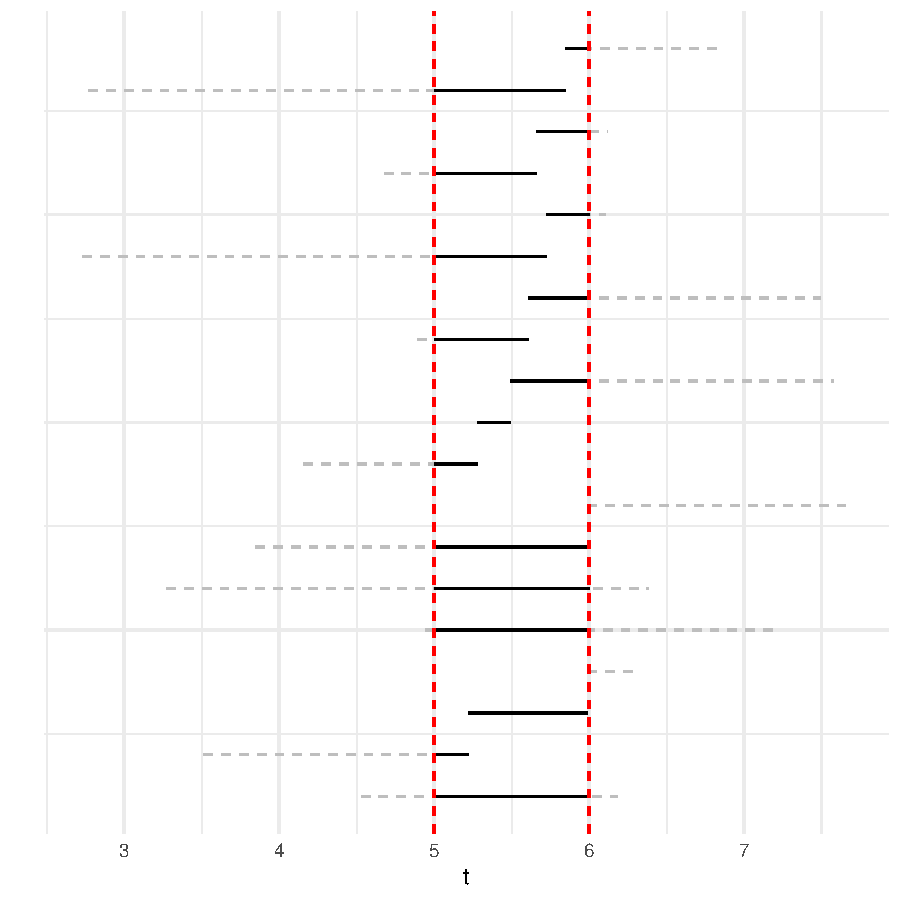
\includegraphics[width=1\textwidth]{./figures/ch-2/sim-data.pdf}
    \caption{The simulated lifetimes data.}
    \label{fig:sim_censored_units}
\end{figure}

\begin{table}
\centering
\caption{\label{tab:sim-cmms-data}The simulated CMMS data for ten units.}
\centering
\begin{tabular}[t]{lrrrrr}
\toprule
Unit & Lifetime & True failure & True install & Observed install & Observed failure\\
\midrule
\cellcolor{gray!10}{1} & \cellcolor{gray!10}{1.66} & \cellcolor{gray!10}{6.18} & \cellcolor{gray!10}{4.53} & \cellcolor{gray!10}{5.00} & \cellcolor{gray!10}{6.00}\\
2 & 1.71 & 5.22 & 3.51 & 5.00 & 5.22\\
\cellcolor{gray!10}{2} & \cellcolor{gray!10}{0.77} & \cellcolor{gray!10}{5.99} & \cellcolor{gray!10}{5.22} & \cellcolor{gray!10}{5.22} & \cellcolor{gray!10}{5.99}\\
2 & 0.31 & 6.31 & 5.99 & 5.99 & 6.00\\
\cellcolor{gray!10}{3} & \cellcolor{gray!10}{2.28} & \cellcolor{gray!10}{7.23} & \cellcolor{gray!10}{4.94} & \cellcolor{gray!10}{5.00} & \cellcolor{gray!10}{6.00}\\
\addlinespace
4 & 3.11 & 6.38 & 3.27 & 5.00 & 6.00\\
\cellcolor{gray!10}{5} & \cellcolor{gray!10}{2.14} & \cellcolor{gray!10}{5.99} & \cellcolor{gray!10}{3.85} & \cellcolor{gray!10}{5.00} & \cellcolor{gray!10}{5.99}\\
5 & 1.69 & 7.68 & 5.99 & 5.99 & 6.00\\
\cellcolor{gray!10}{6} & \cellcolor{gray!10}{1.12} & \cellcolor{gray!10}{5.28} & \cellcolor{gray!10}{4.16} & \cellcolor{gray!10}{5.00} & \cellcolor{gray!10}{5.28}\\
6 & 0.21 & 5.50 & 5.28 & 5.28 & 5.50\\
\addlinespace
\cellcolor{gray!10}{6} & \cellcolor{gray!10}{2.08} & \cellcolor{gray!10}{7.58} & \cellcolor{gray!10}{5.50} & \cellcolor{gray!10}{5.50} & \cellcolor{gray!10}{6.00}\\
7 & 0.71 & 5.61 & 4.90 & 5.00 & 5.61\\
\cellcolor{gray!10}{7} & \cellcolor{gray!10}{1.89} & \cellcolor{gray!10}{7.50} & \cellcolor{gray!10}{5.61} & \cellcolor{gray!10}{5.61} & \cellcolor{gray!10}{6.00}\\
8 & 2.99 & 5.72 & 2.73 & 5.00 & 5.72\\
\cellcolor{gray!10}{8} & \cellcolor{gray!10}{0.39} & \cellcolor{gray!10}{6.11} & \cellcolor{gray!10}{5.72} & \cellcolor{gray!10}{5.72} & \cellcolor{gray!10}{6.00}\\
\addlinespace
9 & 0.98 & 5.66 & 4.68 & 5.00 & 5.66\\
\cellcolor{gray!10}{9} & \cellcolor{gray!10}{0.46} & \cellcolor{gray!10}{6.12} & \cellcolor{gray!10}{5.66} & \cellcolor{gray!10}{5.66} & \cellcolor{gray!10}{6.00}\\
10 & 3.07 & 5.85 & 2.77 & 5.00 & 5.85\\
\cellcolor{gray!10}{10} & \cellcolor{gray!10}{1.03} & \cellcolor{gray!10}{6.88} & \cellcolor{gray!10}{5.85} & \cellcolor{gray!10}{5.85} & \cellcolor{gray!10}{6.00}\\
\bottomrule
\end{tabular}
\end{table}


\subsection{Weakly informative prior} \label{subsec:weibull-model-fits}

I now fit the imputation model to the simulated data in Table~\ref{tab:sim-cmms-data} and compare the resulting posterior with the case where the installation times of the left truncated samples are known and also with the alternative treatment of the unknown exposure histories, which is to discard all of the left truncated samples. I fit these models with a weakly informative, independent priors
\begin{align*}
    \hat{F}_{t_1} \sim & \hbox{N}\left(1.1, 1\right)  \\
    \hat{F}_{t_2} \sim & \hbox{N}\left(1, 1\right).
\end{align*}
The three stan models are available on the GitHub repository. To sample from the posteriors, I use four chains each 1000 iterations long with a burn in of 500. Figure~\ref{fig:joint-post-weibull} shows the three posteriors. Plots (a), (b), and (c) show the joint draws of the two weibull parameters for the fully observed, discarded, and imputed treatment of the left truncated samples respectively. The corresponding CDFs with uncertainty are shown in (d), (e), and (f). The true values of the parameters and the true CDF are plotted in red in the plots. The resulting inference from imputing the installation times of the left truncated samples is almost the exact same as if we had fully observed the left truncated samples. Whereas, discarding the left truncated samples results in a much more diffuse posterior and consequently, more uncertainty around the CDF, particularly for larger exposure times. Next, I refit the models using a slightly more diffuse version of the informative prior shown in Fig.~\ref{fig:kaminskiy-join-priors}~(c) and~(f) which informs the upper tail of the distribution.

\begin{figure}
    \centering
    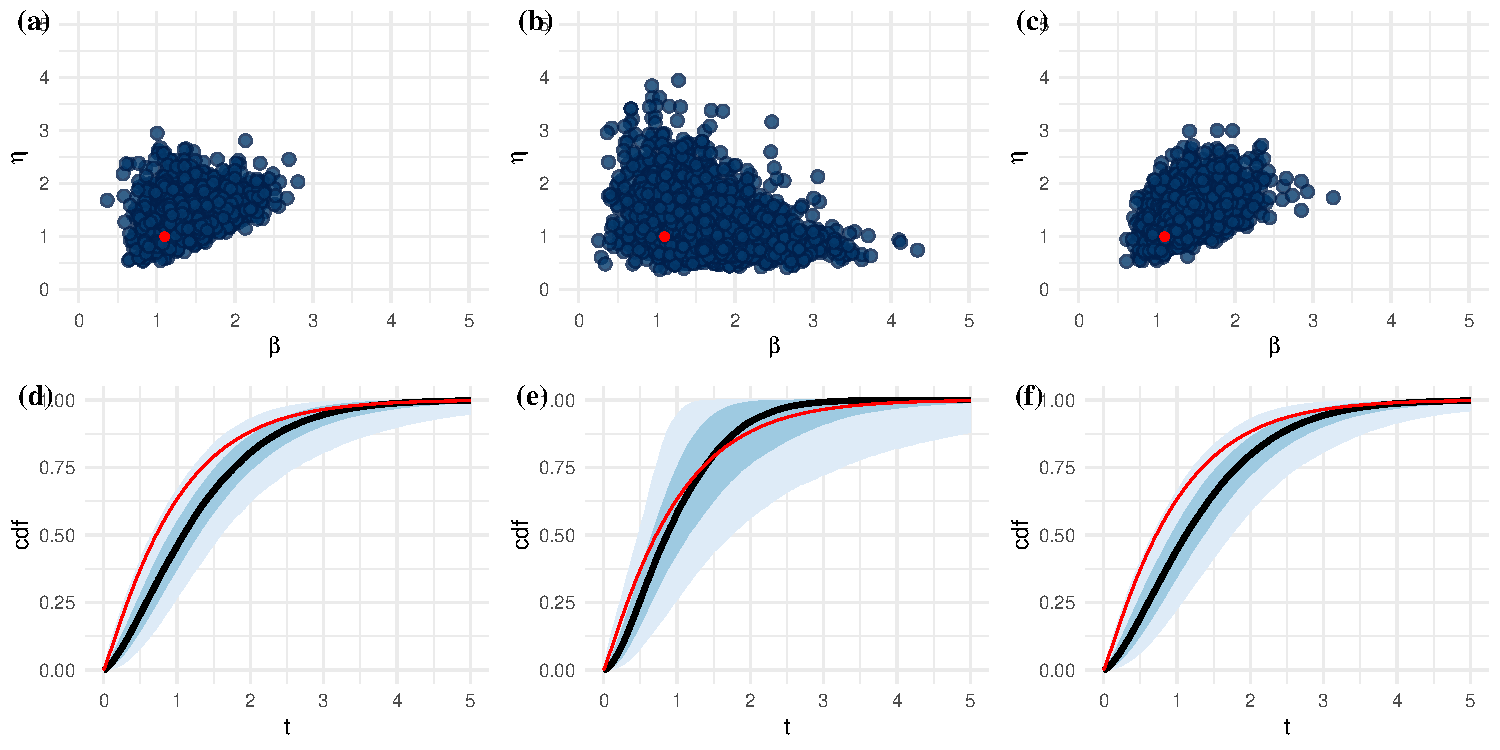
\includegraphics[width=1\textwidth]{./figures/ch-2/joint-posts.pdf}
    \caption{The prior distributions.}
    \label{fig:joint-post-weibull}
\end{figure}

\subsection{Strongly informative prior}

The prior in Fig.~\ref{fig:kaminskiy-join-priors}~(c) and~(f), which elicits information about the CDF at $t_1 = p_{0.80} = 1.54$ and $t_2 = p_{0.95} = 2.71$ encodes an informative prior that strongly informs the Weibull model in the upper tail of the distribution but is sufficiently vague in the lower tail, where the data are strongly informative. Here I refit the weibull models with a slightly more diffuse version of the prior; i.e. I increase the uncertainty around the estimates of the CDF at each elicitation time. The informative prior is
\begin{align*}
    \hat{F}_{t_1} \sim & \hbox{N}^{1}_{0}\left(0.8, 0.1\right)    \\
    \hat{F}_{t_2} \sim & \hbox{N}^{1}_{0}\left(0.95, 0.05\right).
\end{align*}
Using the informative prior, I refit the three models from Section~\ref{subsec:weibull-model-fits}. Once again, I use four chains each 1000 iterations long with a burn in of 500 to sample from the three posteriors. The resulting draws are plotted in (a), (b), and (c) of Figure~\ref{fig:joint-post-weibull-inf} for the fully observed, discarded, and imputed treatment of the left truncated samples respectively. Comparing the posterior of the imputation method (plots~(c)) with the case where the left truncated samples are fully observed (plots~(a)), the resulting inference is again very similar. However, now using the informative prior, the posterior of the case where I have discarded the left truncated samples, plot~(b), is much closer to the other two posteriors than when a vague prior is used. The corresponding posterior CDFs are shown in (d), (e), and (f) of Fig.~\ref{fig:joint-post-weibull-inf}. The uncertainty in all cases has been refined, but most drastically in the upper right part of the CDF. In Fig.~\ref{fig:joint-post-weibull-inf}~(e), the effect of combining a likelihood that informs the CDF at lower exposure times with a prior that informs the CDF at higher exposure times has resulted in a precise estimate of the CDF. 

\begin{figure}
    \centering
    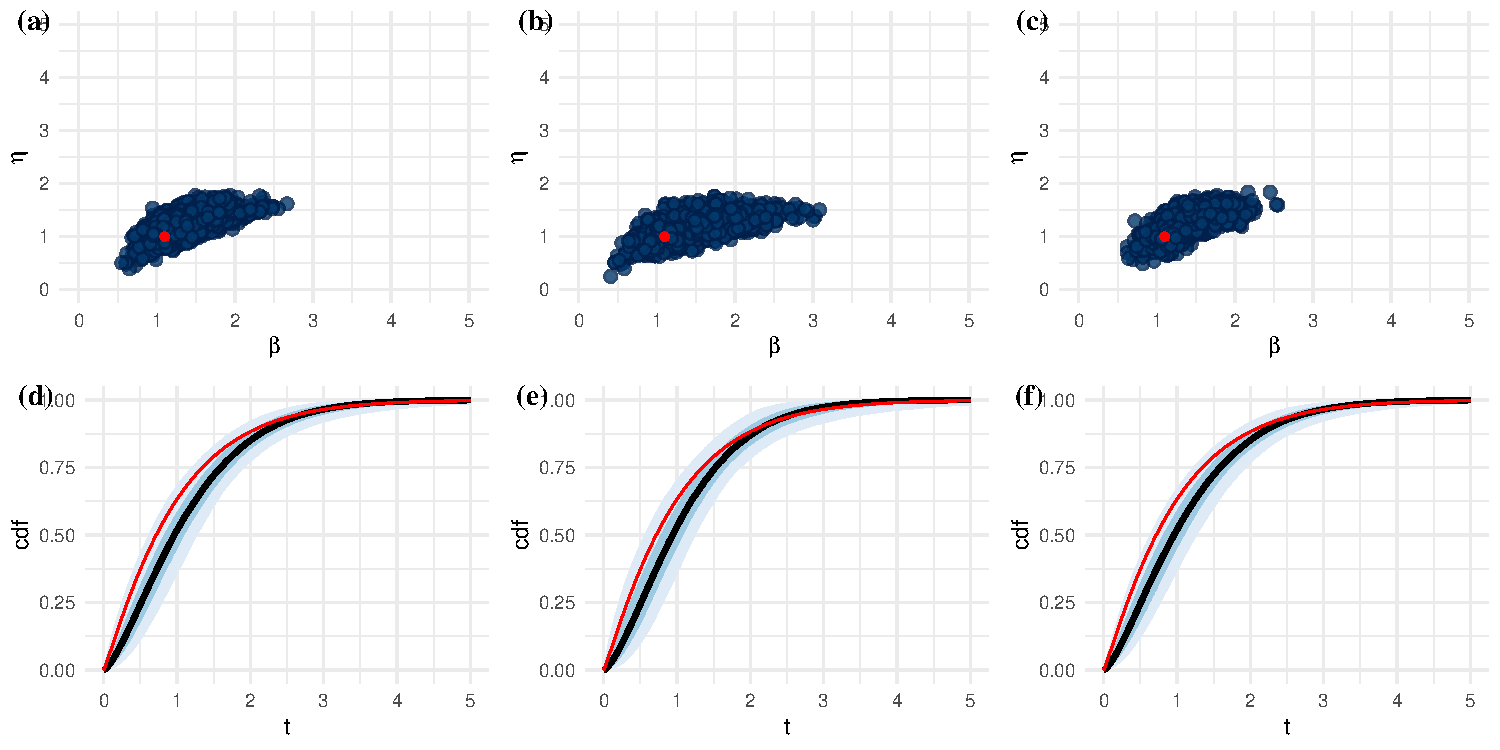
\includegraphics[width=1\textwidth]{./figures/ch-2/joint-posts-inf.pdf}
    \caption{The prior distributions.}
    \label{fig:joint-post-weibull-inf}
\end{figure}

In the implementation of the joint prior that I have used, the prior properly updated. i.e. the observed data have slightly updated our belief about the value of the CDF at both $t_1$ and $t_2$. Figure~\ref{fig:weibull-prior-post-comp} compares the distribution of the posterior draws of $\hat{F}(t_i)$ (gray densities) with the prior (red curves). In the three plots in Fig.~\ref{fig:weibull-prior-post-comp}, the posterior distributions are clearly narrower than the prior; more so at $t_1$. Fitting the Weibull a models for the data in Table~\ref{tab:sim-cmms-data} has shown that, for small samples sizes, in cases where we do not know the exposure history of the left truncated samples the imputation method provides almost equivalent inference to if we had fully observed the left-truncated samples. Further more, if we alternatively `throw away' the left truncated observations this results in an large loss of information, however, this loss can be compensated for if there is prior information about longer lifetimes and this information is properly encoded into a joint prior. Here I have shown one case for a reasonably small sample. Next, I devise a small simulation experiment to more rigorously evaluate the imputation method for the left truncated samples with unknown exposure history.

\begin{figure}
    \centering
    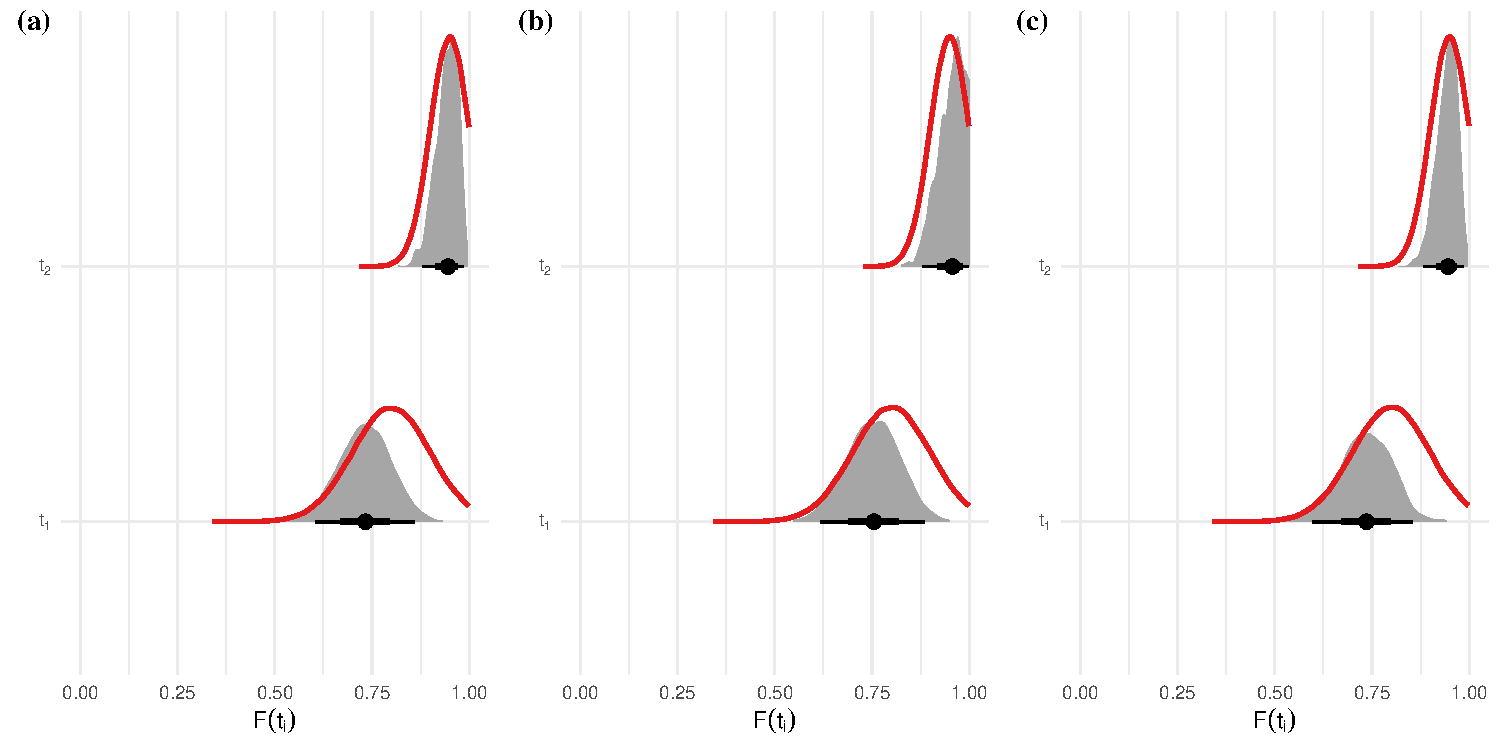
\includegraphics[width=0.8\textwidth]{./figures/ch-2/prior-post-comp.pdf}
    \caption{Comparison of the prior and posterior for $F_{t_1}$ and $F_{t_2}$ to show how both the elicited distributions have been updated.}
    \label{fig:weibull-prior-post-comp}
\end{figure}

%\subsection{Strong likelihood}
%
%When there are many data, and the window is short, there are many lifetimes that are both left truncated, with unknown exposure history, and right censored. In these cases the estimate can be bias. I think this occurs when $t_start$ is not sufficiently far from $t = 0$ for the uniform entry assumption to be valid.
%
\section{Simulation experiments}

To explore the behaviour of the imputation method for left truncated lifetimes with unknown exposure history, I repeat the simulation and model fitting of Section~\ref{sec:weibull-sim-example} for a number of different combinations of the simulation parameters; number of units, start of observation time, and length of observation time. I compare the imputation method---under both a vague and informative prior---with the alternative method of discarding the left truncated observations as well as with the case where the left truncated samples are fully observed (as a ground truth). First I define the factor levels that make up the factor combinations, next I describe the measures of model accuracy that I use to compare the three models, finally, I present the results of the simulation experiments.

\subsection{Factor levels}

I vary three factors when simulating the datasets, each with three levels;
\begin{itemize}
    \item $N$: 10, 100, 500 units
    \item $t_{start}$: 1, 5, 15 mean lifetimes
    \item $t_{end} - t_{start}$: 1, 3, 6 mean lifetimes
\end{itemize}
Increasing the number of units, $N$, increases the sample size, increasing $t_{start}$ increases the range of possible values the left truncated samples with unobserved truncation time could take---and therefore reduces the information they contribute---and increasing the window size, $t_{end} - t_{start}$, increases the number of fully observed lifetimes, the maximum length of the fully observed lifetimes and the number of samples that are both left truncated and right censored. For each factor combination, I perform one hundred simulations, each time fitting all of the three treatments for the left truncated observations with both a vague and informative prior:
\begin{itemize}
    \item model: include lt, discard lt, impute lt
    \item prior: weakly, strongly informative
\end{itemize}
\ldots

\subsection{Accuracy measures}

To compare how well the Bayesian models reclaim the true data generating mechanism, I calculate the Bayesian p-values of the true parameter values---$\beta = 1.1$ and $\eta = 1$---under the fitted posteriors and the $elppd$ of a dataset of one hundred fully observed lifetimes generated from the true weibull distribution. The Bayesian p-value for beta is easily calculated using the posterior draws as
\begin{equation*}
    p_{\beta} = \frac{\sum^{S}_{s = 1}{\beta_{true} \le \beta_s}}{S},
\end{equation*}
similarly the P-value of $\eta$ can be calculated in the same way. If the model posterior is well calibrated, then the p-values from repeating the same simulation should have a uniform distribution. If the parameter estimates are bias then the P-values should on average sit above or bellow 0.5. If the posterior uncertainty is overly diffuse then the p-values will be clustered around 0.5 and if they the uncertainty is too narrow then the P-values will be pushed towards zero or one. The P-value provides a indication that the model is over or under predicting the parameter values, but do not express to what degree.

To determine the scale of any discrepancy, I also calculate the $elppd$ of a new sample of one hundred fully observed lifetimes under the different posteriors. I do this by simulating one hundred datasets, each with one hundred observations, and calculating the expected log likelihood of each simulated dataset and then taking the average,
\begin{equation*}
    elppd_{100} = \frac{\sum_{n = 1}^{100}\frac{1}{S}\sum_{s = 1}^{S}\sum_{i = 1}^{100}f(\tilde{y}_{n, i}|\beta_s, \eta_s)}{100}.
\end{equation*}

\subsection{Results}

The factor combination effects on the p-values.
\begin{itemize}
    \item Description of the plots
    \item Bias in the estimate when the window size is small (I think comes the issue that stan tries to update the truncation time).
    \item There is a small bias in the other cases, these get more visible as the dataset becomes more informative and therefore, the prior more precise.
    \item Despite the slightly biased estimates, the elppd values are remain close. I show this in more detail in the next figure.
\end{itemize}

\begin{figure}
    \centering
    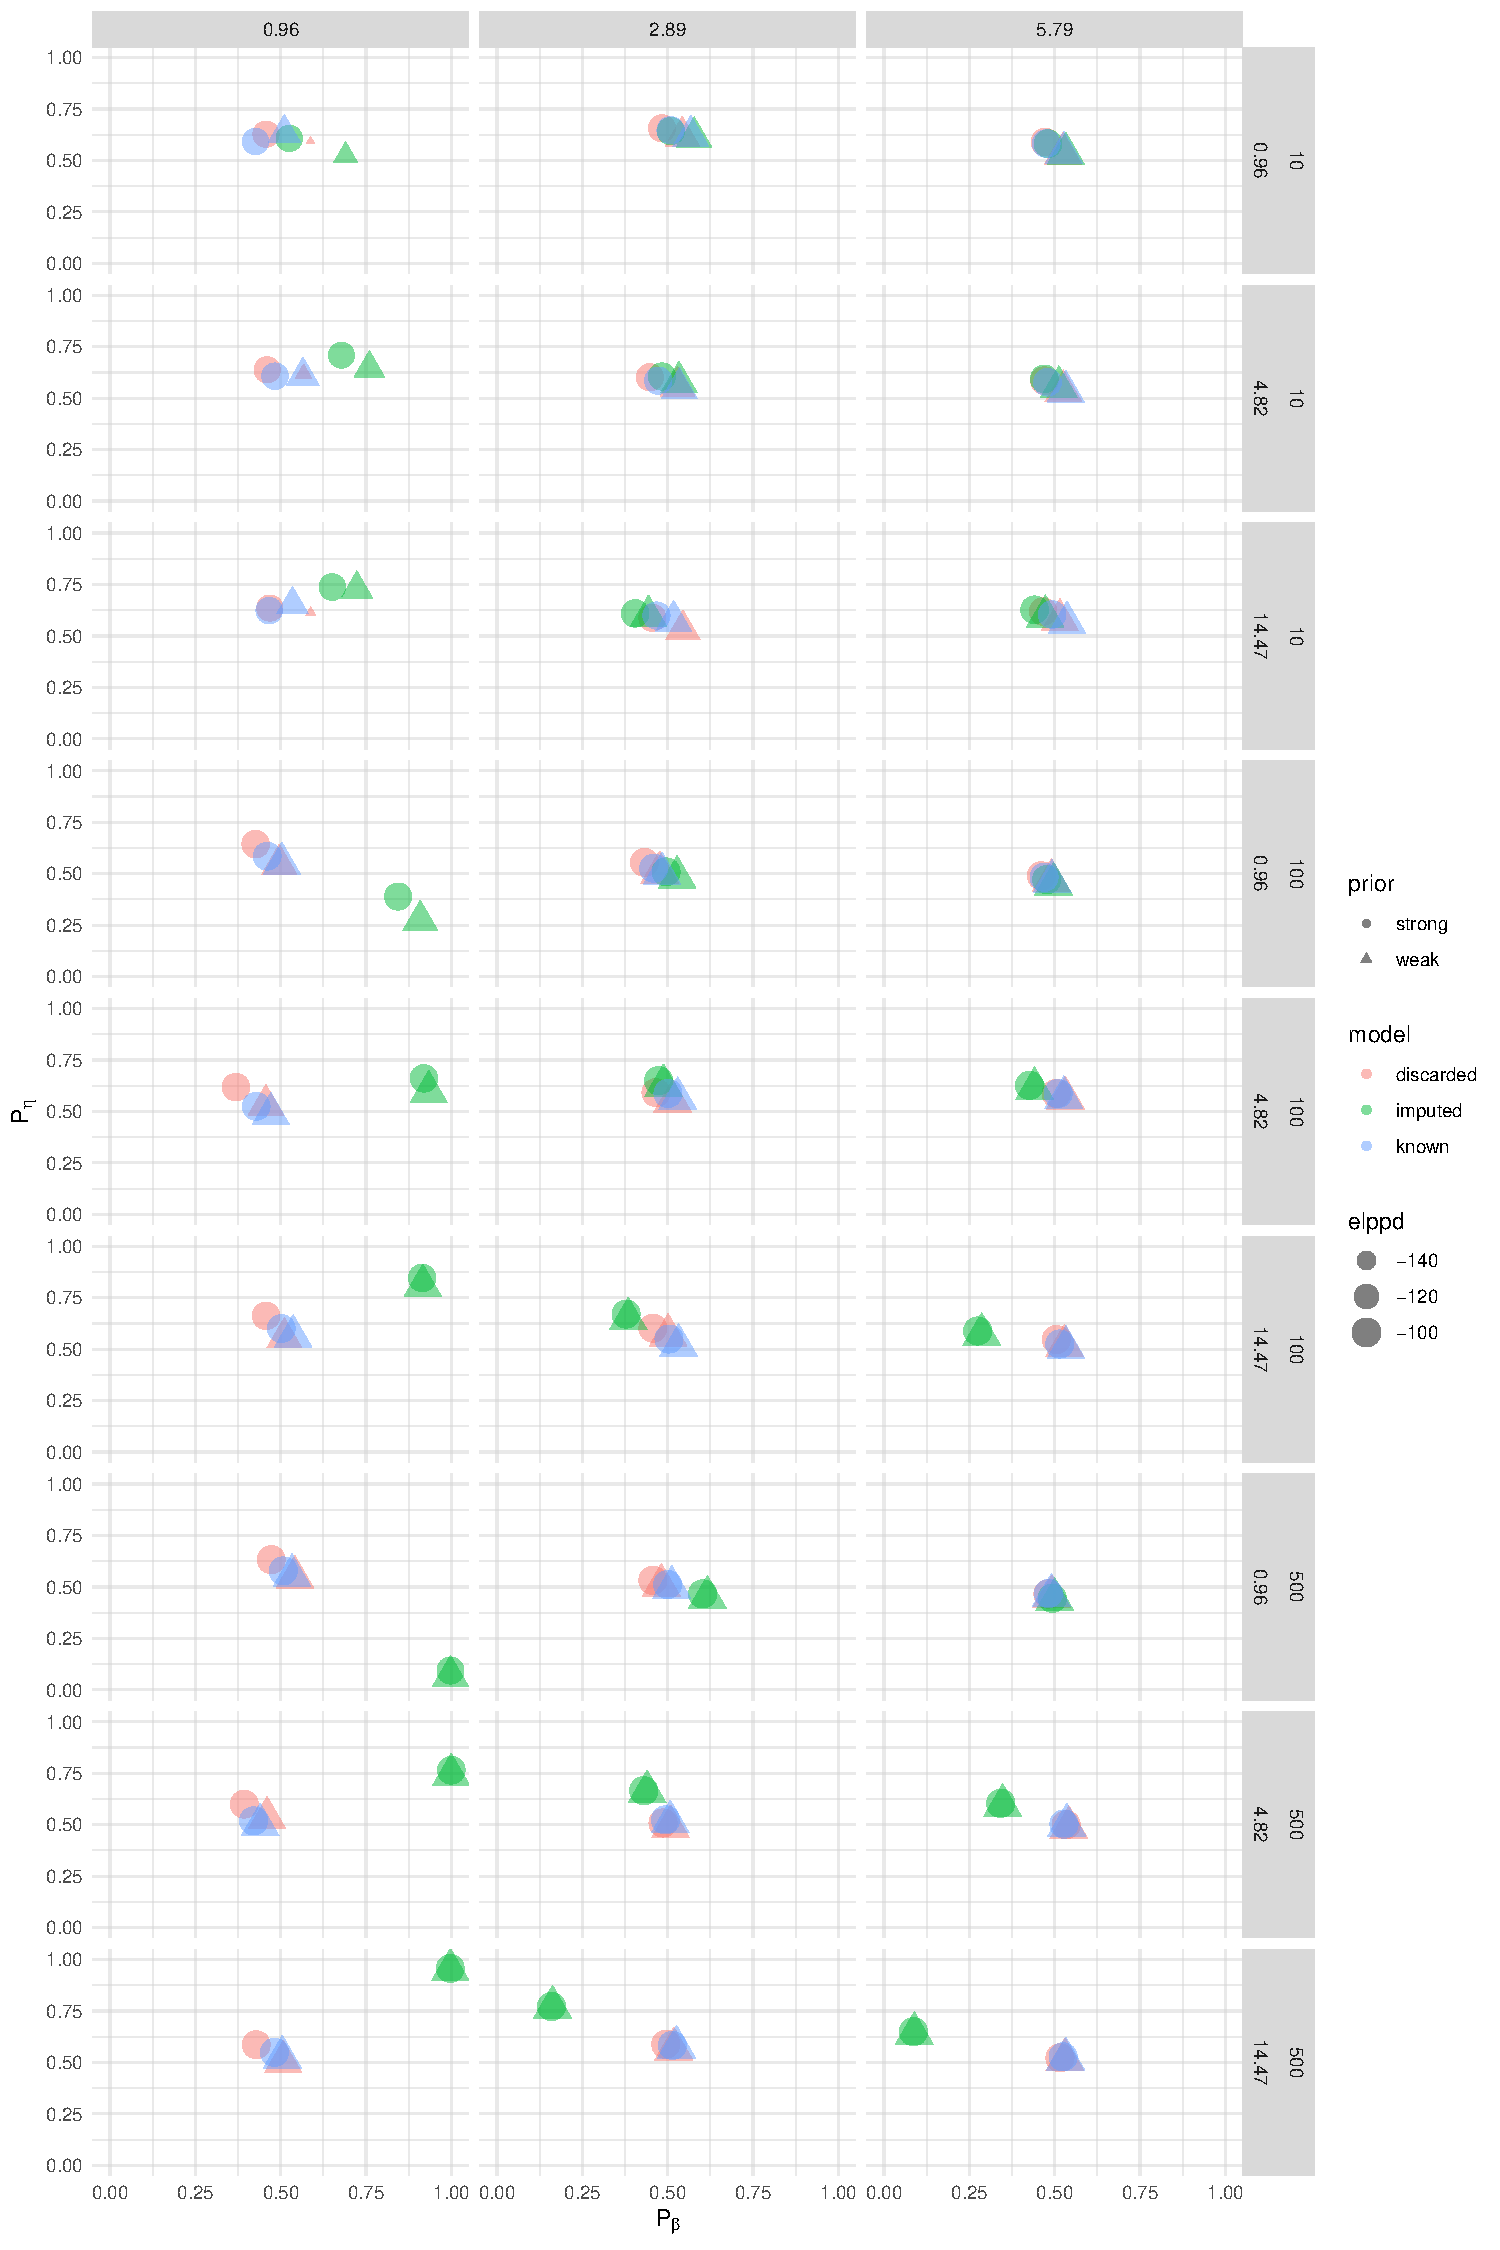
\includegraphics[width=0.8\textwidth]{./figures/ch-2/sim-results-pvalues.pdf}
    \caption{The simulation results}
    \label{fig:sim-study-pvalue}
\end{figure}

The effects on the elppd score. (elppd under the true model is -95.7)
\begin{itemize}
    \item The value is small when the data set is small and the window size is short
\end{itemize}

\begin{figure}
    \centering
    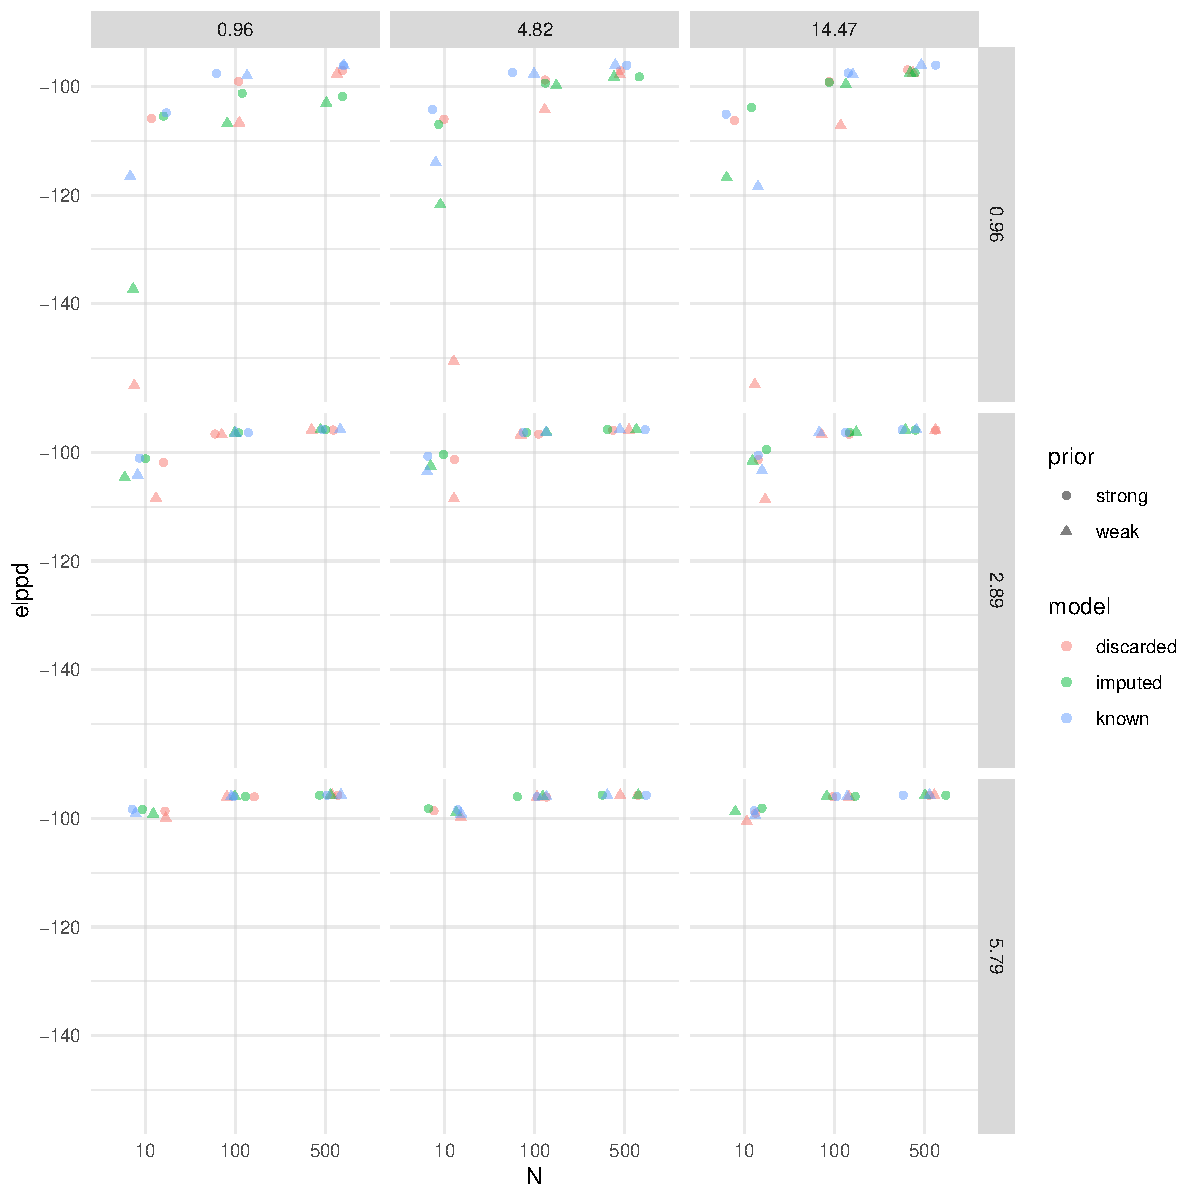
\includegraphics[width=0.8\textwidth]{./figures/ch-2/sim-results-elppd.pdf}
    \caption{The simulation results}
    \label{fig:sim-study-elppd}
\end{figure}

The observed bias is small relative to the noise of the measures.

\section{Concluding remarks}

